\documentclass[conference]{IEEEtran}

\usepackage{cite}
\usepackage{amsmath,amssymb,amsfonts}
\usepackage{algorithmic}
\usepackage{textcomp}
\usepackage{xcolor}

\usepackage{graphicx}
%Path relative to the main .tex file 
\graphicspath{ {./images/} }

\usepackage{verbatim} %for multiline comments

\setlength{\marginparwidth}{2cm}
\usepackage{todonotes} % for TODOs

\def\BibTeX{{\rm B\kern-.05em{\sc i\kern-.025em b}\kern-.08em
    T\kern-.1667em\lower.7ex\hbox{E}\kern-.125emX}}
    
%%% For algorithms 
\usepackage[linesnumbered,ruled,vlined]{algorithm2e}
\SetKwInput{KwInput}{Input}                % Set the Input
\SetKwInput{KwOutput}{Output}              % set the Output
%%% End Algos

\begin{comment}
% make custom headings
\usepackage{titlesec}

\titleformat{\section}
  {\normalfont\fontsize{12}{17}\sffamily\bfseries}
  {\thesection}
  {1em}
  {}
\end{comment}

\begin{document}

\title{\rule{\textwidth}{1pt} Adversarial Training - Paper Outline
\vspace{-1cm} \rule[15pt]{\textwidth}{1pt}}

\author{\IEEEauthorblockN{Moritz Sch{\"u}ler}
\IEEEauthorblockA{\textit{dept. of Informatics} \\
\textit{Technical University Munich}\\
Munich, Germany\\
moritz.schueler@tum.de}
\vspace{-1cm}
}

\maketitle

\begin{IEEEkeywords}
  ML, Adversarial Training, robustness
\end{IEEEkeywords}

\section*{Abstract}
Adversarial training is a technique that tries to achieve robust deep networks. The presented paper provides a conceptual introduction to adversarial training and attacks as well as a review of current methods. Additionally possible directions for future research are presented.

This is the general structure of my review paper about Adversarial Training. It contains the key points that will be outlined in the respective sections. While it's probably not possible to discuss all adversarial training approaches, I plan on describing the concept behind them (maximize margin, ensemble, universal, etc). I will highlight some new recent advancements in detail and discuss their pros and cons. In the end I would present some ideas for future research in this area.


\section{Introduction}

\begin{itemize}
  \item \textbf{Problem and motivation}: Many standard trained neural networks achieve high, even super human performance, however they can be easily fooled with the help of adversarial examples. Adversarial examples are input data with small perturbation applied, which lead a network to predict a wrong class. The root cause is the excessive linearity of trained networks, as can be seen in figure 1 and 2. Figure 1 shows the decision boundaries for a CIFAR10 model, whereas figure 2 shows the presence of adversarial examples in such a linear case. \cite{b6} demonstrated the need for robust models for various practical applications, like autonomous driving. Simply putting a sticker on a stop sign fooled the network to recognize it as a speed limit. 
 % Example lead to research how to defend against but also how to generate such examples.
  \item \textbf{Adversarial attacks}: Adversarial attacks use small perturbations on valid data samples to change the prediction of the classification model. 
  \item \textbf{Adversarial Training}: Adversarial training makes use of self generated adversarial examples instead of the normal data to harden the model against adversarial attacks. It tries to find perturbed samples that get wrongly classified, include them into the training and afterwards adjust the model parameters to get a correct prediction. 
  \item \textbf{Overview}: Short overview of the structure of the paper.
\end{itemize}

\begin{figure}[ht]
  \centering
  \vspace{-0.0cm}
  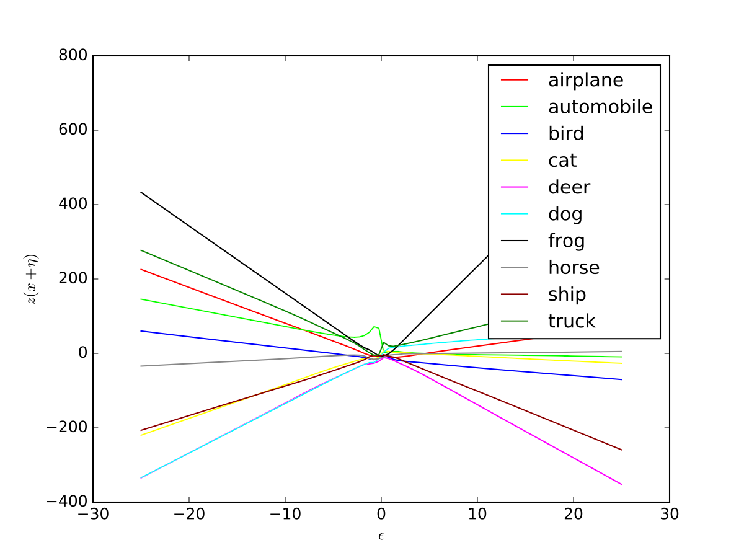
\includegraphics[width=0.48\textwidth]{CIFAR10-decision_boundary.png}
  \label{fig: Decision boundary of a neural network}
  \caption{decision boundary of a neural net trained on CIFAR10} (Baeuml, 2020)
\end{figure}

\begin{figure}[ht]
  \centering
  \vspace{-0.0cm}
  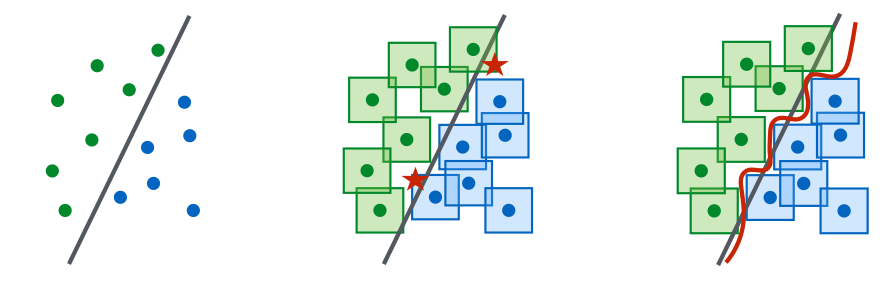
\includegraphics[width=0.48\textwidth]{decision_boundaries.png}
  \label{fig: standard and adversarial decision boundaries}
  \caption{standard and adversarial decision boundaries} (Madry et al. 2019)
\end{figure}

\section{Adversarial Attacks}
\begin{itemize}
  \item \textbf{main idea}: try to find a model that generates samples which result in wrong prediction
  \item \textbf{Properties of adversarial examples}:
  \begin{itemize}
    \item $p(y|x)$ high and $p(y'|x+r)$ high, s.t. $y \neq y' \space \wedge \space r < \epsilon$
    \item $p(y|\tilde{x})$ high s.t. $|x - \tilde{x}|$ large
  \end{itemize}
  \item \textbf{Types}: describe different types of attack
  \begin{itemize}
    % rethinking_softmax_cross_entropy_loss_for_adversarial_robustness
    \item white box: having access to the gradient
    \item grey box: training own model to produce white box attacks
    \item black box: gradient free perturbations
    \item targeted: achieve missclassification for specific sample
    \item untargeted: achieve any missclassification
    \item universal: find perturbation that achieve missclassification for many input samples \\
  \end{itemize}
  \item \textbf{Objective}: The objective is to find a perturbation $\delta$ such that the loss of the classification model is maximized. Usually a threat model $\Delta$ is used for this, which tries to find a $\delta$ within some lp-norm smaller than $\epsilon$, which is a hyperparameter that specifies the strength of the attack. 
  \begin{align*}
    \max_{\delta \in \Delta} \space l(f_{\theta}(x_i + \delta), y_i)  \\
  \Delta = \{\delta : ||\delta||_p \leq \epsilon\} \quad s.t. \quad \epsilon > 0 \\
  \end{align*}
\end{itemize}

\section{Adversarial Training}
\begin{itemize}
  \item \textbf{Main idea}: Train a neural network to be robust against adversarial attacks by using self generated adversarial examples during the training process.\\

  \begin{itemize}
    \item be robust against adversarial attacks
    \item use self generated adversarial examples as training samples
    \item increase non linearity in decision boundary \\
  \end{itemize} 
  
  \item \textbf{Training objective}: The training objective for adversarial training is a two step problem. In the first step the inner maximization is approximated by some threat model, similar or equal to the ones presented for adversarial attacks. Afterwards a variant of gradient descent is used on the model parameters $\theta$. \\
  \begin{align*}
    \min_{\theta} \sum_i \max_{\delta \in \Delta} \space l(f_{\theta}(x_i + \delta), y_i)  \\
  \Delta = \{\delta : ||\delta||_p \leq \epsilon\} \quad s.t. \quad \epsilon > 0 \\
  \end{align*}

  For the gradient descent step the gradient of the inner maximization needs to be computed - can be done using Danskin's Theorem. \\

  \item \textbf{Danskin's Theorem}: The (sub)gradient of a function containing a max term can be found by taking the gradient at the point of the maximum $\delta^{*}$.
  \begin{align*}
    \nabla_{\theta} \max_{||\delta|| \leq \epsilon} l(f_{\theta}(x_i + \delta), y_i) = \nabla_{\theta} l(f_{\theta}(x_i + \delta^{*}(x_i)), y_i)
  \end{align*}

  Danskin's theorem only applies for the exact maximum, but inner term is approximated. Therefore robustness of training is related to how well the approximation is. \\

  \item \textbf{Challenges}: 
  \begin{itemize}
    \item Better inner approximation through multiple steps leads to slow training
    \item Model only good against adversarial attack it was trained on, not always generally robust
  \end{itemize}
\end{itemize}


\section{Methods}

\subsection{Robust Optimization - Standard Adversarial Training} \cite{b2}
The standard approach on adversarial training stems from the view of robust optimization. It formulates the training process as saddle point problem where the adversarial attack tries to maximize the loss whereas the network tries to minimize it.

\begin{align*}
  \min_{\theta} \sum_i \max_{\delta \in \Delta} \space l(f_{\theta}(x_i + \delta), y_i)  \\
\Delta = \{\delta : ||\delta||_p \leq \epsilon\} \quad s.t. \quad \epsilon > 0 \\
\delta^{t+1} = \Pi_{x+S} (\delta^t + \alpha sgn(\nabla_x L(\theta,x,y)))
\end{align*}

\begin{itemize}
  \item FGSM \cite{b9}
  \item K-PGD \cite{b2}: multistep projected FGSM
  \item Free Training \cite{b5}: Mini-batch replay + warm start
  \item Fast Training \cite{b3}: FGSM with random init
  \item GradAlign \cite{b7}: FGSM with Gradient Alignment (refutes random init)
  \item SLAT \cite{b26}: Using latent adversarial perturbations
  \item Bilateral Adversarial Training \cite{b8}: regularize gradient norm
  \item Dual Head Adversarial Training \cite{b24}: use one hat for robustness
  \item Lagrangian objective function \cite{b25}: use lagrangian regularization
\end{itemize}


\subsection{Universal Adversarial Training} \cite{b4}
Universal Adversarial Training is a method that does not try to find a perturbation that works for a single sample but for many samples, hence the name universal. The difference can also be seen in the objective function which iterates over all samples in the inner term. As it tries to find a universal perturbation it is more constrained than the standard approach and hence leads to a less robust model, while reducing the training time.

\begin{align*}
  \min_{\theta} \sum_i \max_{\delta \in \Delta} \space \frac{1}{N} \sum_{i=1}^N \space l(f_{\theta}(x_i + \delta), y_i) \quad s.t. \quad ||\delta||_p \leq \epsilon
\end{align*}

\begin{itemize}
  \item Universal Adversarial perturbations \cite{b10}
  \item universal Adversarial Training with class-wise perturbations \cite{b11}
  \item Deep Fool
  \item Defending Against Universal Perturbations With Shared Adversarial Training \cite{b12}
  % -> 20 times slower than normal training
  \item Defense against Universal Adversarial Perturbations \cite{b13}
\end{itemize}

\subsection{Margin Maximization} \cite{b1}
Margin Maximization is a method that tries to maximize the distance between each sample and its nearby decision boundary. Intuitively this makes the model more robust as an adversarial example is a slight perturbation that changes the model outcome and is usually a sample that is closest to the original data but on the other side of the decision boundary. Thus by maximizing said distance it is harder to generate adversarial examples with small perturbations and therefor increasing robustness.

\begin{align*}
  \min_{\theta} \sum_i \max \{0, d_{max} - d_\theta(x_i, y_i)\} \\
  d_\theta(x,y) = ||\delta^*|| = min ||\delta|| \quad \text{s.t.} \quad \delta: L_\theta^{01}(x+\delta, y) = 1
\end{align*}

\begin{itemize}
  \item MMA Training: Direct input space margin maximization through adversarial training\cite{b1}
  \item Deep Defense: Adversarial Margin Maximization Networks \cite{b14}
  \item Large Margin Deep Networks for Classification \cite{b15}
  \item Margin Maximization for Robust Classification using Deep Learning \cite{b16}
  \item MACER: Attack-free and scalable robust training via maximizing certified radius \cite{b17}
  \item Lipschitz-Margin Training: Scalable Certification of Perturbation Invariance for Deep Neural Networks \cite{b18}
\end{itemize}

\subsection{Adversarial Logit Pairing} \cite{b19, b20}
Adversarial logit pairing consists of the usual cross entropy loss for training and an additional logit similarity loss. This second term measures the difference with an L-norm between the logit of a clean sample and the corresponding adversarial sample.

\begin{align*}
  loss: J(M, \theta) + \lambda \frac{1}{m} \sum_{i=1}^m L(f(x^{(i)}; \theta), f(\tilde{x}^{(i)}; \theta))
\end{align*}

\subsection{Ensemble Adversarial Training} \cite{b23}
Ensemble adversarial training uses an ensemble of models for the generation of the adversarial examples used for training. To be efficient, it uses static pre-trained models using the fact that most adversarial examples are model agnostic.


\subsection{Distillation} \cite{b21, b22}
Distillation is a technique to reduce the dimensionality of a network without loss of accuracy, but in the setting of adversarial training it is used to get a better generalization and this means intuitively a more robust model. It first uses a network to generate output distributions for each sample and afterwards using these to train a second network.  

\begin{align*}
  \arg \min_{\theta_F} - \frac{1}{|\chi|} \sum_{X \in \chi} \sum_{i \in 0..N} F_i(X) log F_i^d(X) \\
\end{align*}

\begin{comment}
The general intuition behind the technique
is to extract class probability vectors produced by a first DNN
or an ensemble of DNNs to train a second DNN of reduced
dimensionality without loss of accuracy.
This intuition is based on the fact that knowledge acquired
by DNNs during training is not only encoded in weight
parameters learned by the DNN but is also encoded in the
probability vectors produced by the network. Therefore, distil-
lation extracts class knowledge from these probability vectors
to transfer it into a different DNN architecture during training.
To perform this transfer, distillation labels inputs in the training
dataset of the second DNN using their classification predic-
tions according to the first DNN.
\end{comment}

\section{Review}
In this section, the previously presented training methods are compared (e.g. in a table) based on the following criteria:
\begin{itemize}
  \item \textbf{Normal Accuracy}: which methods provide the highest accuracy
  \item \textbf{Robust Accuracy against different attacks}: which methods provide the highest robust accuracy
  \item \textbf{Combined Accuracy}: which methods provide the highest combined accuracy
  \item \textbf{Efficient Training}: which method has the highest accuracy in relation to the training time
  \item \textbf{Steadiness} which method is robust against most of the attacks
  \item \textbf{Application} which method to use in which scenario \\
\end{itemize}


\section{Future Research}
\begin{itemize}
  \item \textbf{Multi Head Training}: Train multiple heads for clean input, adversarial examples within the data distribution and far away from it. Optionally add a classification network/layer to decide which class corresponds to a given input at test time. \cite{b24}
  \item \textbf{Variable $\epsilon$}: Adjust $\epsilon$ to every training sample for standard adversarial training. \cite{b1}
  \item \textbf{Random Lp-Norm}: Randomize the used Lp-Norm for the inner maximization to increase average robustness over all Lp-Norms. 
  \item \textbf{Neural architecture search}: Use NAS to determine architectures specifically for robust training. \\
\end{itemize}

%raise concerns that this still doesnt mean that network learns same features as a human


\begin{thebibliography}{00}

  \bibitem{b1} Gavin Weiguang Ding, Yash Sharma, Kry Yik Chau Lui, Ruitong Huang: MMA Training: Direct input space margin maximization through adversarial training. 2019.
  \bibitem{b2} Aleksander Madry, Aleksandar Makelov, Ludwig Schmidt et al.: Towards Deep Learning Models Resistant to Adversarial Attacks. 2019.
  \bibitem{b3} Eric Wong, Leslie Rice, J. Zico Kolter: Fast is better than Free: Revisiting adversarial training. 2020.
  \bibitem{b4} Ali Shafahi, Mahyar Najibi, Zheng Xu et al. Universal Adversarial Training. 2020.
  \bibitem{b5} Ali Shafahi, Mahyar Najibi, Amin Ghiasi, Zheng Xu, John Dickerson, Christoph Studer, Larry S Davis, Gavin Taylor, and Tom Goldstein. Adversarial training for free! 2019.
  \bibitem{b6} Eykholt, K., Evtimov, I., Fernande, E., Li, B., Rahmati, A., Xiao, C., Prakash, A., Kohno, T., and Song, D. Robust physicalworld attacks on deep learning visual classification. 2018.
  \bibitem{b7} Maksym Andriushchenko, Nicolas Flammarion. Understanding and Improving
  Fast Adversarial Training. 2020.
  \bibitem{b8} Jianyu Wang, Haichao Zhang. Bilateral Adversarial Training: Towards Fast Training of More Robust Models Against Adversarial Attacks. 2019.
  \bibitem{b9} Ian J Goodfellow, Jonathon Shlens, and Christian Szegedy. Explaining and harnessing adversarial examples. 2014.
  \bibitem{b10} Seyed-Mohsen Moosavi-Dezfooli, Alhussein Fawzi, Omar Fawzi,Pascal Frossard. Universal adversarial perturbations. 2017.
  \bibitem{b11} Philipp Benz, Chaoning Zhang, Adil Karjauv, In So Kweon. Universal adversarial training with class-wise perturbations. 2021.
  \bibitem{b12} Chaithanya Kumar Mummadi, Thomas Brox, Jan Hendrik Metzen. Defending Against Universal Perturbations With Shared Adversarial Training. 2019.
  \bibitem{b13} Naveed Akhtar, Jian Liu, Ajmal Mian. Defense against Universal Adversarial Perturbations. 2018.
  \bibitem{b14} Ziang Yan, Yiwen Guo, and Changshui Zhang. Adversarial Margin Maximization Networks. 2019.
  \bibitem{b15} Gamaleldin F. Elsayed, Dilip Krishnan, Hossein Mobahi, Kevin Regan, Samy Bengio. Large Margin Deep Networks for Classification. 2018.
  \bibitem{b16} Alexander Matyasko, Lap-Pui Chau. Margin Maximization for Robust Classification using Deep Learning. 2017.
  \bibitem{b17} Runtian Zhai, Chen Dan, Di He, Huan Zhang, Boqing Gong, Pradeep Ravikumar, Cho-Jui Hsieh, Liwei Wang. MACER: Attack-Free and scalable robust training via maximization certified radius. 2020.
  \bibitem{b18} Yusuke Tsuzuku, Issei Sato, Masashi Sugiyama. Lipschitz-Margin Training: Scalable Certification of Perturbation Invariance for Deep Neural Networks. 2018.
  \bibitem{b19} Harini Kannan, Alexey Kurakin, Ian Goodfellow. Adversarial Logit Pairing. 2018.
  \bibitem{b20} Marius Mosbach, Maksym Andriushchenko, Thomas Trost, Matthias Hein, Dietrich Klakow. Logit Pairing Methods Can Fool Gradient-Based Attacks. 2019.
  \bibitem{b21} Nicolas Papernot, Patrick McDaniel, Xi Wu, Somesh Jha, Ananthram Swami. Distillation as a Defense to Adversarial Perturbations against Deep Neural Networks. 2016.
  \bibitem{b22} Nicholas Carlini, David Wagner. Defensive Distillation is Not Robust to Adversarial Examples. 2016.
  \bibitem{b23} Florian Tramèr, Alexey Kurakin, Nicolas Papernot, Ian Goodfellow, Dan Boneh, Partick McDaniel. Ensemble Adversarial Training: Attacks and Defenses. 2020.
  \bibitem{b24} Yujing Jiang , Xingjun Ma, Sarah Monazam Erfani, James Bailey. Dual Head Adversarial Training. 2021.
  \bibitem{b25} Mohammad Azizmalayeri, Mohammad Hossein Rohban. Lagrangian Objective Function Leads to Improved Unforeseen Attack Generalization in Adversarial Training. 2021.
  \bibitem{b26} Geon Yeong Park, Sang Wan Lee. Reliably fast Adversarial Training via latent adversarial perturbation. 2021.

\end{thebibliography}

\newpage

\section{Appendix}

\end{document}
